%Research Plan - 20%
\section{Research Plan} 
\label{sec:research}

Re-state the problem you are trying to solve and then explain how you plan to solve it. Is it designing a new visualization? Is it designing a new library?  Is it running a controlled experiment? Is it something else?

Note this is a {\em plan}. The plan may change as you make discoveries during your project. However, you must describe what your plan is assuming everything goes as expected. If there are some parts of the plan where you could run into difficulties, state what those difficulties are and what alternative measures you could take should those difficulties arise.

You may refer to other sections so as not to repeat yourself -- for example, referencing Section~\ref{sec:background}.

You may want to use figures to illustrate your point, such as Figure~\ref{fig:sample}.

\begin{figure}[h]
 \centering % avoid the use of \begin{center}...\end{center} and use \centering instead (more compact)
 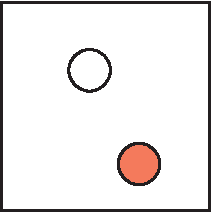
\includegraphics[width=1.5in]{figs/sample}
 \caption{Figure illustrating some proposed designs.}
 \label{fig:sample}
\end{figure}

\subsection{Data}
\label{sec:data}

Describe the data here. Describe whether you already have access to the data and if not, what is required to obtain the data. If you don't already have the data, explain how long it will take to retrieve it. 

\subsection{Evaluation}
\label{sec:eval}

Describe your plan for evaluating your work during this project.

Then, describe how you would evaluate the work beyond the timeframe of the project. Without time constraints, what would you do? Do you have the resources (people, time, equipment, data, money) to implement this plan in the future? Does your plan for evaluating your work during the project serve as a first step to this evaluation?

\subsection{Technology}
\label{sec:tech}

Describe what technologies you intend to use (e.g., programming languages, platforms, existing libraries) and why they make sense for your project. Do they serve your users better than other technologies? Are you able to take advantage of existing work/libraries for your domain with this technology rather than HTML/CSS/JS and d3.js?  

\subsection{Timeline}
\label{sec:timeline}

Adapt the milestones for the class project to the specifics of your project, describe them in this section, and summarize in Table~\ref{tab:milestones}.  You may set intermediate milestones, but you should make it clear what you will have accomplished by the progress update milestone (due Oct. 29, 2020).  Use paragraphs to make it clear what the milestone means, for example:

\paragraph{Milestone 1} Description

\paragraph{Milestone 1} Description

These milestones can include many subgoals.  If you are developing a new technique or visualization, you should have a preliminary idea of the design.  You may want to consider developing a prototype or preliminary design by the progress update step.  Any data needed to support initial findings or background work should be cited and discussed.  If you are doing a literature review or taxonomy, you should have a preliminary list of papers you will review as well as an explanation of the methodology used to generate such a list.  If your evaluation requires scaffolding code to run things, or human subjects to test things, you can describe when you will set these up.

By the progress update stage, there should be initial results of the first chunk of work that needs to be done.  In most projects with implementation this will involve a working data reader and at least one visualization, library feature, or study question type working. As you will need a report at this stage, be sure to set up milestones that will provide you with sufficient material to develop your report and update your plan, if necessary.   The demonstration should run with minimal effort and the code should be included in the repository.

Later milestones (after the progress update stage) can include a variety of stages included a complete prototype of the project artifacts,  such as a visualization tool, a visualization library, a working study with experimental objects and stimuli complete, or completed literature annotations with an categorization schema. The plan for evaluation especially should be updated indicating the plan for milestone five and any preliminary work in the design of that evaluation.


Additionally, a full report of the project as a whole should be included as a milestone.



\begin{table}[h]
%% Table captions on top in journal version
 \caption{Project Milestones}\vspace{1ex} % the \vspace adds some space after the top caption
 \label{tab:milestones}
 \scriptsize
 \centering % avoid the use of \begin{center}...\end{center} and use \centering instead (more compact)
   \begin{tabular}{r|r}
     Milestone & Description (\%)\\
   \hline
     Date & Summary Description \\
     Date & Summary Description \\
     October 29 & Progress Update \\
     Date & Summary Description \\
     December 8 & Final Report Completed \\
   \end{tabular}
\end{table}

